
\Sec{On summoning penguins with}{The Ti\textit{k}Z Package}

\begin{frame}[fragile,c]
\vspace*{1ex}%
\begin{layout-full}
\begin{center}
\begin{onlyenv}<2|handout:1>
\begin{tikzexample}
\begin{tikzpicture}
   \draw (0,0) -- (1,0);
\end{tikzpicture}
\end{tikzexample}
\end{onlyenv}
\begin{onlyenv}<3|handout:1>
\begin{tikzexample}
\begin{tikzpicture}
   \draw (0,0) -- (1,0)
               -- (2,1);
\end{tikzpicture}
\end{tikzexample}
\end{onlyenv}
\begin{onlyenv}<4|handout:1>
\begin{tikzexample}
\begin{tikzpicture}
   \draw (0,0) -- (1,0)
               -- ++(2,1);
\end{tikzpicture}
\end{tikzexample}
\end{onlyenv}
\begin{onlyenv}<5|handout:2>
\begin{tikzexample}
\begin{tikzpicture}
   \draw (0,0) -- (1,0)
               |- ++(2,1);
\end{tikzpicture}
\end{tikzexample}
\end{onlyenv}
\begin{onlyenv}<6|handout:2>
\begin{tikzexample}
\begin{tikzpicture}
   \draw (0,0) -- (1,0)
       to[bend right] ++(2,1);
\end{tikzpicture}
\end{tikzexample}
\end{onlyenv}
\begin{onlyenv}<7|handout:2>
\begin{tikzexample}
\begin{tikzpicture}
   \draw (0,0) -- (1,0)
       to[out=0,in=180] ++(2,1);
\end{tikzpicture}
\end{tikzexample}
\end{onlyenv}
\begin{onlyenv}<8|handout:3>
\begin{tikzexample}
\begin{tikzpicture}
   \draw[->] (0,0) -- (1,0)
       to[out=0,in=180] ++(2,1);
\end{tikzpicture}
\end{tikzexample}
\end{onlyenv}
\begin{onlyenv}<9|handout:3>
\begin{tikzexample}
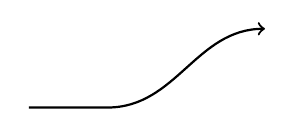
\begin{tikzpicture}
   \draw[->,thick] (0,0) -- (1,0)
       to[out=0,in=180] ++(2,1);
\end{tikzpicture}
\end{tikzexample}
\end{onlyenv}
\begin{onlyenv}<10|handout:3>
\begin{tikzexample}
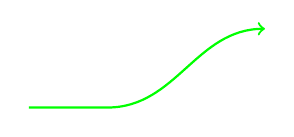
\begin{tikzpicture}
   \draw[->,thick,green] (0,0) -- (1,0)
       to[out=0,in=180] ++(2,1);
\end{tikzpicture}
\end{tikzexample}
\end{onlyenv}
\begin{onlyenv}<11|handout:4>
\begin{tikzexample}
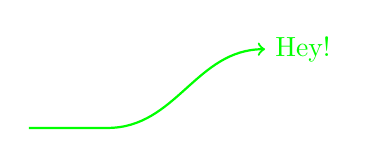
\begin{tikzpicture}
   \draw[->,thick,green] (0,0) -- (1,0)
       to[out=0,in=180] ++(2,1)
       node[right] {Hey!};
\end{tikzpicture}
\end{tikzexample}
\end{onlyenv}
\begin{onlyenv}<12|handout:4>
\begin{tikzexample}
\begin{tikzpicture}
   \node (a) at (1,1) {A};
\end{tikzpicture}
\end{tikzexample}
\end{onlyenv}
\begin{onlyenv}<13|handout:4>
\begin{tikzexample}
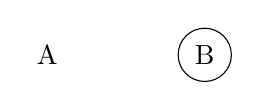
\begin{tikzpicture}
   \node (a) at (1,1) {A};
   \node[circle,draw] (b) at (3,1) {B};
\end{tikzpicture}
\end{tikzexample}
\end{onlyenv}
\begin{onlyenv}<14|handout:5>
\begin{tikzexample}
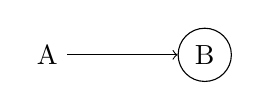
\begin{tikzpicture}
   \node (a) at (1,1) {A};
   \node[circle,draw] (b) at (3,1) {B};
   \draw[->] (a) -- (b);
\end{tikzpicture}
\end{tikzexample}
\end{onlyenv}
\begin{onlyenv}<15|handout:5>
\begin{tikzexample}

\begin{tikzpicture}
   \fill (1,.75) circle[radius=2mm]
      node[white] {X};
\end{tikzpicture}
\end{tikzexample}
\end{onlyenv}
\begin{onlyenv}<16|handout:6>
\begin{tikzexample}

\begin{tikzpicture}
   \fill (1,.75) circle[radius=2mm]
      node[white] {X};
   \node[circle,fill,text=white]
      at(3,.75) {X};
\end{tikzpicture}
\end{tikzexample}
\end{onlyenv}
\end{center}
\end{layout-full}
\end{frame}